\documentclass[a4paper,11pt,titlepage]{bxjsarticle}
\usepackage[dvipdfmx]{graphicx}
\usepackage{listings}
\usepackage{amsmath}
\usepackage{fancybox,ascmac}
\usepackage{url}
\title{画像処理}
\author{175751C 宮城孝明}
\date{\today}
\begin{document}
\maketitle
\tableofcontents
\clearpage
\section{課題1}
\subsection{ソースコード}
\lstinputlisting[language=python, numbers=left, breaklines=true, basicstyle=\ttfamily\footnotesize,
  frame=single, caption=課題1, label=sample]{ImageShow2.py}
 \subsection{実行結果}
 \begin{figure}[htbp]
 \begin{minipage}{0.5\hsize}
  \begin{center}
   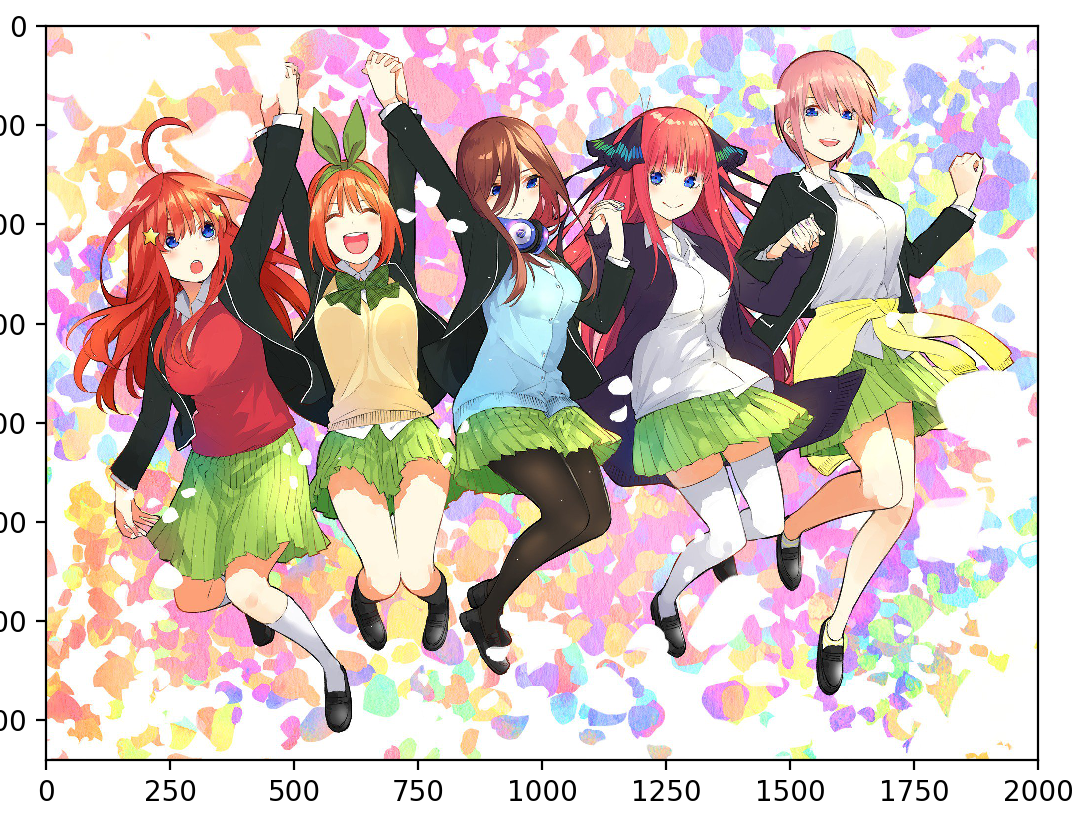
\includegraphics[width=70mm]{kadai1.png}
  \end{center}
  \caption{0~10秒後と15秒~}
  \label{fig:one}
 \end{minipage}
 \begin{minipage}{0.5\hsize}
  \begin{center}
   
\includegraphics[width=70mm]{kadai1-1.png}
  \end{center}
  \caption{11~15秒}
  \label{fig:two}
 \end{minipage}
\end{figure}
\section{課題2}
\subsection{ソースコード}
\lstinputlisting[language=python, numbers=left, breaklines=true, basicstyle=\ttfamily\footnotesize,
  frame=single, caption=課題3, label=sample]{ImageZahyo.py}
\subsection{実行結果}
\begin{figure}[htbp]
 \begin{center}
  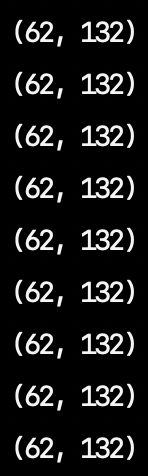
\includegraphics[width=18mm]{kadai2.png}
 \end{center}
 \caption{課題2の図}
 \label{fig:one}
\end{figure}
\section{課題3}
\subsection{ソースコード}
\lstinputlisting[language=python, numbers=left, breaklines=true, basicstyle=\ttfamily\footnotesize,
  frame=single, caption=課題3, label=sample]{ImageZahyoShow.py}
\subsection{実行結果}
\begin{figure}[htbp]
 \begin{center}
  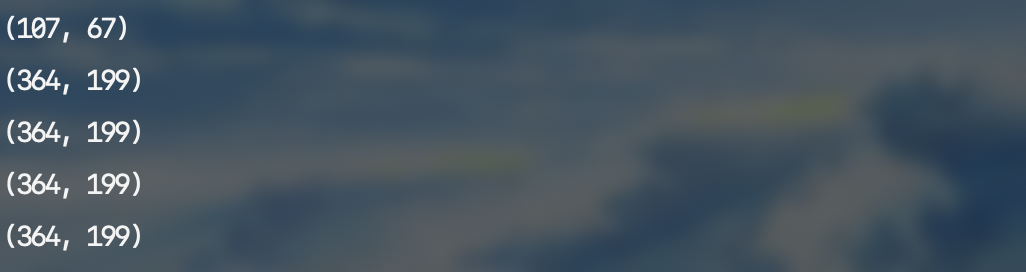
\includegraphics[width=100mm]{kadai3.png}
 \end{center}
 \caption{課題2の図}
 \label{fig:one}
\end{figure}

\section{課題4}
\subsection{ソースコード}
\lstinputlisting[language=python, numbers=left, breaklines=true, basicstyle=\ttfamily\footnotesize,
  frame=single, caption=課題4, label=sample]{ImageGasoShow.py }
\subsection{実行結果}
\begin{figure}[htbp]
 \begin{center}
  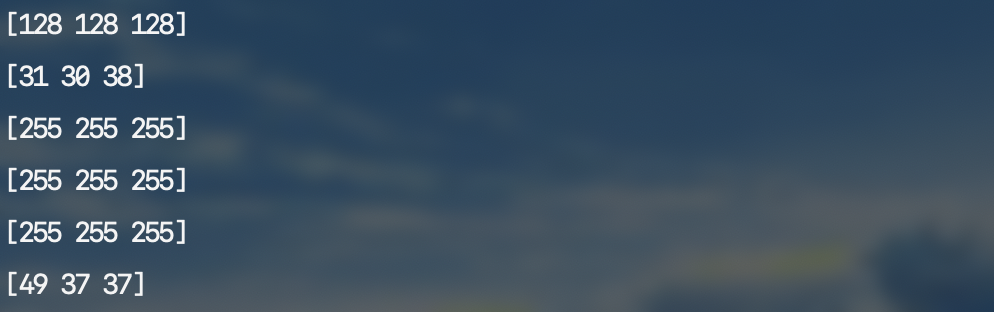
\includegraphics[width=100mm]{kadai4.png}
 \end{center}
 \caption{課題2の図}
 \label{fig:one}
\end{figure}

\section{課題5}
\subsection{ソースコード}
\lstinputlisting[language=python, numbers=left, breaklines=true, basicstyle=\ttfamily\footnotesize,
  frame=single, caption=課題5, label=sample]{ImageSizeShow.py}
\subsection{実行結果}
\begin{figure}[htbp]
 \begin{center}
  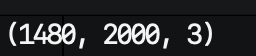
\includegraphics[width=100mm]{kadai5.png}
 \end{center}
 \caption{課題2の図}
 \label{fig:one}
\end{figure}

\section{課題6}
\subsection{ソースコード}
\lstinputlisting[language=python, numbers=left, breaklines=true, basicstyle=\ttfamily\footnotesize,
  frame=single, caption=課題6, label=sample]{ImageEncloseShow.py }
\subsection{実行結果}
\begin{figure}[htbp]
 \begin{center}
  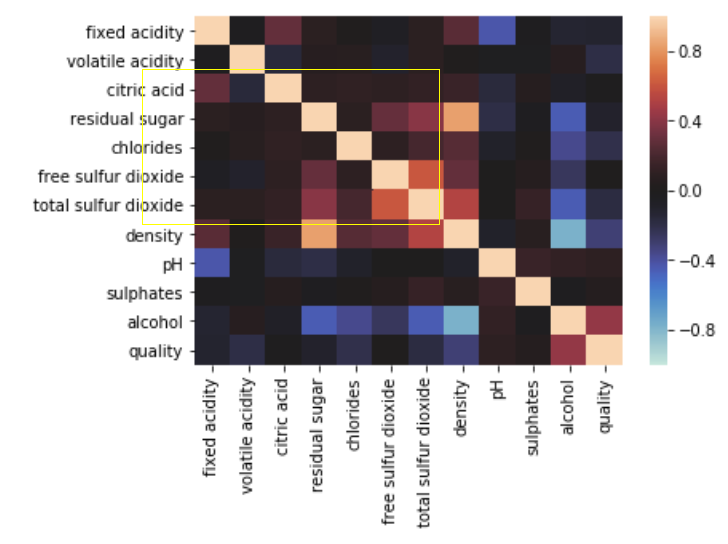
\includegraphics[width=50mm]{sample2.png}
 \end{center}
 \caption{課題2の図}
 \label{fig:one}
\end{figure}
\end{document}


